\section{Method}
\label{SECII}\label{sec:method}
\subsection{The standard approach: matched filtering}

Searches for gravitational waves from compact binary coalescences typically employ matched filter banks \cite{findchirppaper}.  Potential inspiral signals are continuously parameterized by time, amplitude, phase, and a set of intrinsic source parameters $\theta$, which in this paper we shall take to consist of the two component masses of a binary, $\theta = (m_1, m_2)$.  Let $h_+(\theta)$ and $h_\times(\theta)$ be, respectively, the `$+$' and `$\times$' polarization gravitational wave signals that would arise from a fiducial face-on binary at some distance.  Because, for inspiral signals, $h_+$ and $h_\times$ are nearly in quadrature, they are generally combined into a single complex-valued template $h = h_+ + i h_\times$.

The detection procedure for just one set of intrinsic source parameters $\theta$ starts by {\em whitening} the measurement data stream $x$.  This involves finding a linear filter that renders the detector's noise \textsc{iid} and Gaussian.  This filter is applied to the measurement, yielding the whitened data stream $x^\mathrm W$.  The same linear filter is applied to the template $h(\theta)$, yielding the whitened template $h^\mathrm W (\theta)$.  The matched filter is the normalized cross-correlation of $h^\mathrm W$ and $x^\mathrm W$, \editorial{After introducing the $\star$ notation for cross correlation, must we define it for continuous and discrete time?}
$$
\rho(\theta) = \frac{h^\mathrm W (\theta) \star x^\mathrm W}{|h^\mathrm W (\theta)|}.
$$
This is called the signal to noise ratio, or \textsc{snr}.  The detection statistic is the modulus of this, $|\rho(\theta)|$, which has a $\chi^2$ distribution with 2 degrees of freedom in the absence of signal.%, and it indicates the probability of a signal being present \cite{wainstein:1962}\editorial{Comment about probability doesn't seem relevant.}.

To construct a filter bank, matched filters are realized for discrete signal parameters $\theta_1,\, \theta_2,\, \cdots$, $\theta_N$, such that any possible signal will have a maximum cross-correlation of at least 0.97 with at least one template.  \editorial{Citation needed for template placement procedure?}  Such a template bank is said to have a 97\% {\em minimum match}.  This technique is designed so that an inspiral signal can be detected without any prior knowledge of its intrinsic parameters: at most 3\% of the \textsc{snr} is lost by a signal's parameters not exactly coinciding with a template's.  A trigger is reported for the template parameters $\theta_i$ and time $t$ for which $|\rho|$ is a maximum over some moving interval in $\theta$ and $t$.

\subsubsection{Latency and overhead}

The matched filter bank can be implemented with finite impulse response (\textsc{fir}) filters.  \textsc{fir} filters are perfectly suited for realtime detection, because they do not introduce any latency at all.  However, \textsc{fir} filters are very expensive: for $N$ templates of $M$ samples each, a \textsc{fir} matched filter bank costs $\mathcal O(M N)$ operations per sample.

Much more commonly, the matched filter bank is implemented using \textsc{fft} convolutions, costing only $\mathcal O(M \lg N)$ \editorial{$\lg$ is $\log_2$. Explain nomenclature? Switch to $\log_2$?} per sample but having a latency of at least $M$ samples.  For example, for a bank of $1\,\mathrm{ks}$ templates sampled at $4096\,\mathrm{Hz}$, the \textsc{fft} implementation requires about about $2.2 \times 10^4$ times fewer floating point operations per sample than the \textsc{fir} implementation.  However, the \textsc{fft} implementation has a latency of at least $1\,\mathrm{ks}$.

This presents a dilemma: it seems that low latency detection using the \textsc{fir} implementation is prohibitively expensive, whereas computational cheap detection with the \textsc{fft} method comes with minutes to hours of latency.

In the rest of the section, we will describe a detection strategy that makes use of some very general properties of inspiral template banks in order to evaluate a matched filter bank with far lower computational cost than the \textsc{fir} method and far less latency than the \textsc{fft} method.

\subsection{Selectively reducing the sample rate of the data and template waveforms}

Our first innovation is based upon the common knowledge that gravitational waveforms from the inspiral stage of compact binary coalescences are chirps: they are quasi-monochromatic and slowly evolving in frequency.

\editorial{The time slice boundary notation is a little awkward and different identifiers are used in a few places in the source code.  It would be nice to clean that up.}  It is possible to strike a balance between the low latency of the \textsc{fir} filter method and the low overhead of the \textsc{fft} method by breaking the templates into disjoint time intervals, or {\em time slices}.  The outputs of the filters for all of the time slices are delayed by the appropriate numbers of samples and then summed to produce the \textsc{snr}s for original templates in the template bank.  Each time slice may be implemented using either \textsc{fir} filters or \textsc{fft} convolution.  If the $i$th time slice spans the times $[-t_\mathrm{end}^i, -t_\mathrm{start}^i)$ relative to the time of coalescence, then the latency is $\max \, (2 (t_\mathrm{end}^i - t_\mathrm{start}^i) - t_\mathrm{start}^i)$, where the maximum is taken over all time slices that are implemented using \textsc{fft} convolution.
\editorial{It may be worth pointing out that time-slicing buys you latency even
without exploiting time-frequency structure. The downsampling really just buys
you throughput. It may even be worth renaming the section.}

We can exploit the time-frequency structure of the templates by processing each time slice at a reduced sample rate.  In the quadrupole approximation~\cite{finn1993}, the frequency of gravitational radiation resulting from the inspiral of two compact objects evolves according to
\begin{equation}
\label{eq:fgw}
f = \frac{1}{\mathcal{\pi M}} \left[ \frac{5}{256}\frac{\mathcal{M}}{-t} \right]^{3/8}
\end{equation}
where $\mathcal{M}$ is the chirp mass and $t$ is the time relative to the coalescence of the binary~\cite{kidder1992, blanchet2002, findchirppaper, hanna2009}. \editorial{Way too many citations here.} Typically the template is truncated at some time before coalescence, corresponding to a finite frequency which is often chosen to be the frequency at the innermost stable circular orbit, $f_\mathrm{final} = f_\mathrm{ISCO} = 4400 \, M_\odot / M$.

Applying the relationship $f/f_\mathrm{final} = (t_\mathrm{final}/t)^{3/8}$ it is possible to design time slices such that the templates are critically sampled at monotonically decreasing sample rates.  The data stream is downsampled to many different sample rates, then filtered in each time slice, then upsampled to a high common sample rate, and summed.  In order to work efficiently with radix-2 \textsc{fft}s, sample rates and sample counts for time slices are both constrained to be powers of 2.

\editorial{I didn't mention the upsampling and downsampling overhead, but I included it in my calculation.  Should I describe this here, in an appendix, or in a publicly available tech note in the \textsc{dcc}?} An example time slice design satisfying these constraints for a $1.4 - 1.4 \, M_{\odot}$ is shown in table~\ref{table:time_slices} below.  For this example, the latency for this time slice design is just $\input{time_slice_latency.tex}$ even if all of the time slices are implemented with the \textsc{fft} method.  This set of time slices will require $\input{time_slice_ops_firslice.tex}$ operations per sample per template, compared with $\input{time_slice_ops_conv.tex}$ for pure \textsc{fft} cross-correlation without time slices, or $\input{time_slice_ops_td.tex}$ for the \textsc{fir} filter method without time slices.

\begin{table}[!h]
\caption{Example of critically sampled, power-of-2 time slices for a $1.4 - 1.4 \, M_{\odot}$ template extending from $f_\mathrm{low} = 10 \, \mathrm{Hz}$ to $f_\mathrm{ISCO} = 1571\, \mathrm{Hz}$ with a time frequency structure given by ($\ref{eq:fgw})$.}
\label{table:time_slices}
\begin{minipage}[c]{0.5\textwidth}
\centering
\includegraphics[trim = 3cm 0cm 1.5cm 0cm, scale=0.4]{time_slices.pdf}
\end{minipage}
\begin{minipage}[c]{0.3\textwidth}
\centering
\input{time_slices.tex}
\end{minipage}
\end{table}

\editorial{\textsc{mbta} should be cited in the introduction.}  This idea has been demonstrated by the Virgo Collaboration's \textsc{mbta} pipeline~\cite{beauville2006,beauville2008}, which operated in a low-latency mode during \textsc{ligo}'s sixth science run and Virgo's second science run in 2010.

A similar procedure can be applied for any signal family that is piecewise band-limited, as long as the time-frequency evolution is understood, either symbolically as in equation~(\ref{eq:fgw}), or numerically.

\subsection{Reducing the number of filters with the singular value decomposition}

Our second innovation exploits the fact that the templates in inspiral template banks are, by design, highly correlated.  It is possible to greatly reduce the number of matched filters required to achieve a particular minimum match by designing an appropriate set of orthonormal {\em basis templates}.  A purely numerical technique based on the singular value decomposition (\textsc{svd}) is demonstrated by the authors in~\cite{Cannon:2010p10398}.

\editorial{I'm sweeping the complex nature of the templates under the rug here.  Is it OK to regard our packing of the real and imaginary parts of the \textsc{svd} as an implementation detail?  It makes the math a little more concise.}  One may regard a bank of $N$ discretely sampled templates of length $M$ samples, $h^\mathrm W(\theta_i; t_j) = [\mathbf H]_{ij} = H_{ij}$, as a matrix.  The singular value decomposition is an exact factorization that exists for any matrix such that
\begin{equation}
\label{eq:svd-exact}
H_{ij} = [\mathbf {V \Sigma U}]_{ij} = \sum_{k=1}^{N} v_{ik} \sigma_k u_{kj},
\end{equation}
where $\mathbf V$ and $\mathbf U$ are both unitary matrices and $\mathbf \Sigma$ is a diagonal matrix.  For our purposes, we associate the rows of $\mathbf U$ with a minimal set of basis templates, which become the kernels of basis filters.  These filters give rise to the orthogonal \textsc{snr}s, $[\mathbf \rho^\perp]_k = \rho_k^\perp = \mathbf{U}_k \star x^\mathsf{W}$.  The rows of $\mathbf{V \Sigma}$ become reconstruction coefficients that map linear combinations of the orthogonal \textsc{snr}s from the basis filters back onto \textsc{snr}s for the original templates of interest: $\rho_i = \sum_k [\mathbf V \mathbf \Sigma]_{ik} \rho_k^\perp$.

In many applications of the \textsc{svd}, including ours, the matrix can be well approximated by truncating the summation in equation~(\ref{eq:svd-exact}) at $L \ll N$:
\begin{equation}
H_{ij}^\prime = \sum_{k=1}^{L} v_{ik} \sigma_k u_{kj}
\end{equation}
The cumulative sum of squares of the {\em singular values}, $\sigma_k$, measures the Frobenius norm of the approximation, such that
\begin{equation}
\frac{\| \mathbf H^\prime \|}{\| \mathbf H \|} = \left(\sum_{k=1}^{L} |\sigma_k|^2\right)^{1/2} \left(\sum_{k=1}^{N} |\sigma_k|^2\right)^{-1/2}.
\end{equation}
This is also called the \textsc{svd} tolerance.  In our application, it relates to how much \textsc{snr} is lost by discarding $N - L$ of the basis filters with the lowest singular values.

\begin{comment}

% Rewritten above.

It is clear that in order to reduce the cost of a low latency search for
compact binaries of unknown mass we need to reduce the number of convolutions
necessary to find the gravitational-wave signal.  Rather than filter the
$i$ templates corresponding to binaries of different component masses it is
possible to find a basis set of fewer filter $u_j$ that can be linearly combined
to reproduce $\rho_i$ to some accuracy.  For the remainder of this section
we will drop the explicit time dependence of the convolution and recognize
that the snr for any point in time is simply the innerproduct between a
template waveform vector ${\bf \hat{h}_i}$ and a vector of the detector data 
${\bf \hat{s}}$, $\rho_i = ({\bf \hat{h}_i}|{\bf \hat{s}})$.  
The goal is to have
\begin{equation}
\label{eq:linear_combination_of_snr}
\rho_i = \sum_{j=1}^{N'} M_{ij} ({\bf \hat{u}_j}|{\bf \hat{s}})
\end{equation}
where the number of inner products is reduced from $N$ to $N'$. In order to
find the basis set ${\bf u_j}$ we use the singular value decomposition of
the matrix 
${H_{ik}} = \{{\bf \hat{h}_1}, {\bf \hat{h}_2}, ...{\bf \hat{h}_N}\}$. Where
$i$ is the index over the template number and $k$ is the index over sample 
points. The singular value decomposition factors a matrix such that
\begin{equation}
\label{eq:svd}
{H_{ik}} = {A_{ij}\,B_{jl}\,U_{lk}}
\end{equation}
The matrix ${B_{jl}}$ is a diagonal matrix of singular values ranked in
order of importance of reconstructing the original matrix ${H_{ik}}$.
However since a search for binary inspirals only needs  waveform accuracy to a
few percent to be successful it is possible to make an approximate 
reconstruction of ${H_{ik}}$ 
\begin{equation}
\label{eq:svdapprox}
{H_{ik}} \approx {A_{ij}\,B'_{jl}\,U_{lk}}
\end{equation}
where the rank of ${B'_{jl}}$ is less than the rank of ${B_{jl}}$.
This reduces the number of rows in ${U_{lk}}$.  Now we have a 
new basis of template waveforms derived from ${U_{lk}} = \{{\bf \hat{u}_1}, {\bf \hat{u}_2}, ...{\bf \hat{u}_{N'}}\}$ and can write 
(\ref{eq:linear_combination_of_snr})
\begin{eqnarray}
\label{eq:svdsnr}
\rho_i &=& \sum_{j=1}^{N'} A_{il}\,B'_{lj} ({\bf \hat{u}_j}|{\bf \hat{s}}) \nonumber \\
       &=& \sum_{j=1}^{N'} M_{ij} ({\bf \hat{u}_j}|{\bf \hat{s}})
\end{eqnarray}

\end{comment}

\editorial{This passage, from the original draft, sounds confrontational to me, but these are good citations.  Can we tone it down or move it elsewhere?}  This result differs from other work that models gravitational-wave chirp signals in approximate ways~\cite{Chassande-Mottin2006, Candes2008, BuonannoChenVallisneri:2003a} by starting with an exact representation of the desired template family and producing a rigorous approximation with a tunable accuracy.  

\subsection{Composite detection statistic and hierarchical detection}

Although the \textsc{svd} allows us to reduce the number of matched filters, this comes at the price of having to perform a matrix multiplication by the reconstruction matrix $\mathbf {V \Sigma}$ at every sample.  In some circumstances, this matrix multiplication may be more expensive than applying the orthogonal matched filters.

\editorial{We have an old block diagram of our pipeline, but it takes up a lot of space.  A new, more compact one that uses conventional signal-flow diagram symbols would be nice.}  Further speedup may be gained in a hierarchical detection scheme.  In general, the orthogonal \textsc{snr}s alone provide some indication of whether any template in the original template bank is likely to have a large \textsc{snr}.  Consider some composite detection statistic that is a scalar function of the orthogonal \textsc{snr}s, $\Gamma(\rho_1^\perp, \rho_2^\perp, \cdots, \rho_L^\perp)$.  Suppose that we can infer the distribution of $\Gamma$ for a data stream with the signal present or with the signal absent.  Then we may use a threshold crossing of $\Gamma$ to trigger the conditional application of the expensive reconstruction matrix only during the times when a signal is likely to be present.

The composite detection statistic that we employ is a weighted sum of squares, $\Gamma = \sum_{k=1}^L w_k (\rho_k^\perp) ^ 2$, with the particular weights
\begin{equation}
w_k = \frac{\sigma_k^2}{\sigma_k^2 + N / A^2}.
\end{equation}
\editorial{We now have a pretty good description of time slices, the SVD, and conditional reconstruction.  We still need to tie it all together.}Here, $A$ is a desired \textsc{snr} scale that is set by the analyst.  As the authors show in ~\cite{svd-compdetstat}, this choice of weights has a better receiver operating characteristic for a signal of \textsc{snr}~=~$A$ than some other obvious choices, $w_k = \sigma_k^2$ or $w_k = 1$.

\begin{comment}

% Fold this into SVD discussion.

%\subsection{Detection statistic}
It is not necessary to reconstruct the SNR of all templates in order to 
determine if a signal is present.  By thresholding on the sum of squares
of the orthoganal decomposition described above it is possible to answer
whether or not an inspiral like event is in the data.  Then only 
potentially interesting times can be reconstructed on a sample by sample 
basis.  Following the ideas in~\cite{Anderson:2000yy} we employ a detection
statistic as
\begin{equation}
\label{eq:stat}
\Gamma^2 = \sum_{l} \sum_{j} {B'_{lj}}^2 {({\bf \hat{u}_j}|{\bf \hat{s}})}^2
\end{equation}

\end{comment}

\begin{comment}

% We aren't using this chi square test.

\subsection{Signal consistency check}
After reconstructing the SNR of an individual template it is possible to 
to check that the components along the SVD basis were consistent with 
expectation by performing a $\chi^2$ fit to the decomposition.  
\begin{equation}
\label{eq:chisq}
\chi^2_i = \sum_j {[({\bf \hat{u}_j}|{\bf \hat{s}}) - \rho_i / M_{ij}]}^2
\end{equation}

\end{comment}

\begin{comment}

% I think that this part can be swalled into the computational costs discussion above.

\subsection{Comparison of computational costs and latency}
Convolutions are best done with the use of the Fast Fourier Transform (FFT).
However there is an inherent latency in performing convolutions this way. This
section describes the computational cost and latency of FFT convolutions, time 
domain (TD) convolutions and TD convolutions with SVD.  

Convolving one filter with data using FFTs involves 
$\mathcal{O}[10 N_s \log_2(N_s)]$
floating point operations where $N_s$ is the number of sample points in
the data being convolved and results in $N_s - N_f$ samples of usable output.  
In comparison time domain convolutions require
$\mathcal{O}[N_s N_f]$ where $N_f$ is the number of sample points in the
filter.  The FFT is faster to compute when $N_f > 10 \log_2(N_s)$.  However
the FFT has an inherent latency of $\mathcal{O}[N_s/f_s]$ seconds, where
$f_s$ is the sample rate when minimally overlapping FFTs are computed. It is
possible to reduce the latency of the FFT by performing vastly overlapping
FFTs.  The cost of such a procedure would be 
$\mathcal{O}[10 N_o N_s \log_2(N_s)]$.  Thus for comparable computational
cost where $N_f \approx 10 N_o \log_2(N_s)$ the latency of the FFT method 
would be $\mathcal{O}[N_s/f_s/N_o]$ seconds.  Depending on the task at hand,
latency requirements and computational costs can dictate what procedure to
use.

\end{comment}

\begin{comment}

% Do we want to spend this much copy on the whitener?
% What matters is that we have picked a low-latency whitening procedure.

\subsection{Data Whitening}
Matched filtering the SVD basis vectors has motivated a decoupling of the
whitening routine from the matched filtering engine. This was necessary in
order weight templates appropriately by whitening them before the SVD
calculation, and, as such, we have also moved the data whitening outside the
match filter engine. We have chosen to whiten the data using a running
geometric average of the PSD computed by Hann windowing 8 second buffers of
data and using 50\% overlapping buffers. The running geometric average is
updated once per buffer from a median of the recent PSDs. We find that this
algorithm is extremely fast to converge to an accurate PSD and also very robust
against glitches. This is demonstrated below where we have injected
band-limited white noise burst with a central frequency of 150 Hz, a bandwidth
of 100 Hz, a time duration of 0.2 seconds, and a injection density of one
injection every $100/\pi \approx 32$ seconds. At this density we find there
should only ever be one injection affecting the median history so the glitches
should minimally affect PSD estimation as can be seen by comparing the local
RMS amplitude between injections to that without injections.

\begin{center}
\resizebox{0.9\textwidth}{!}{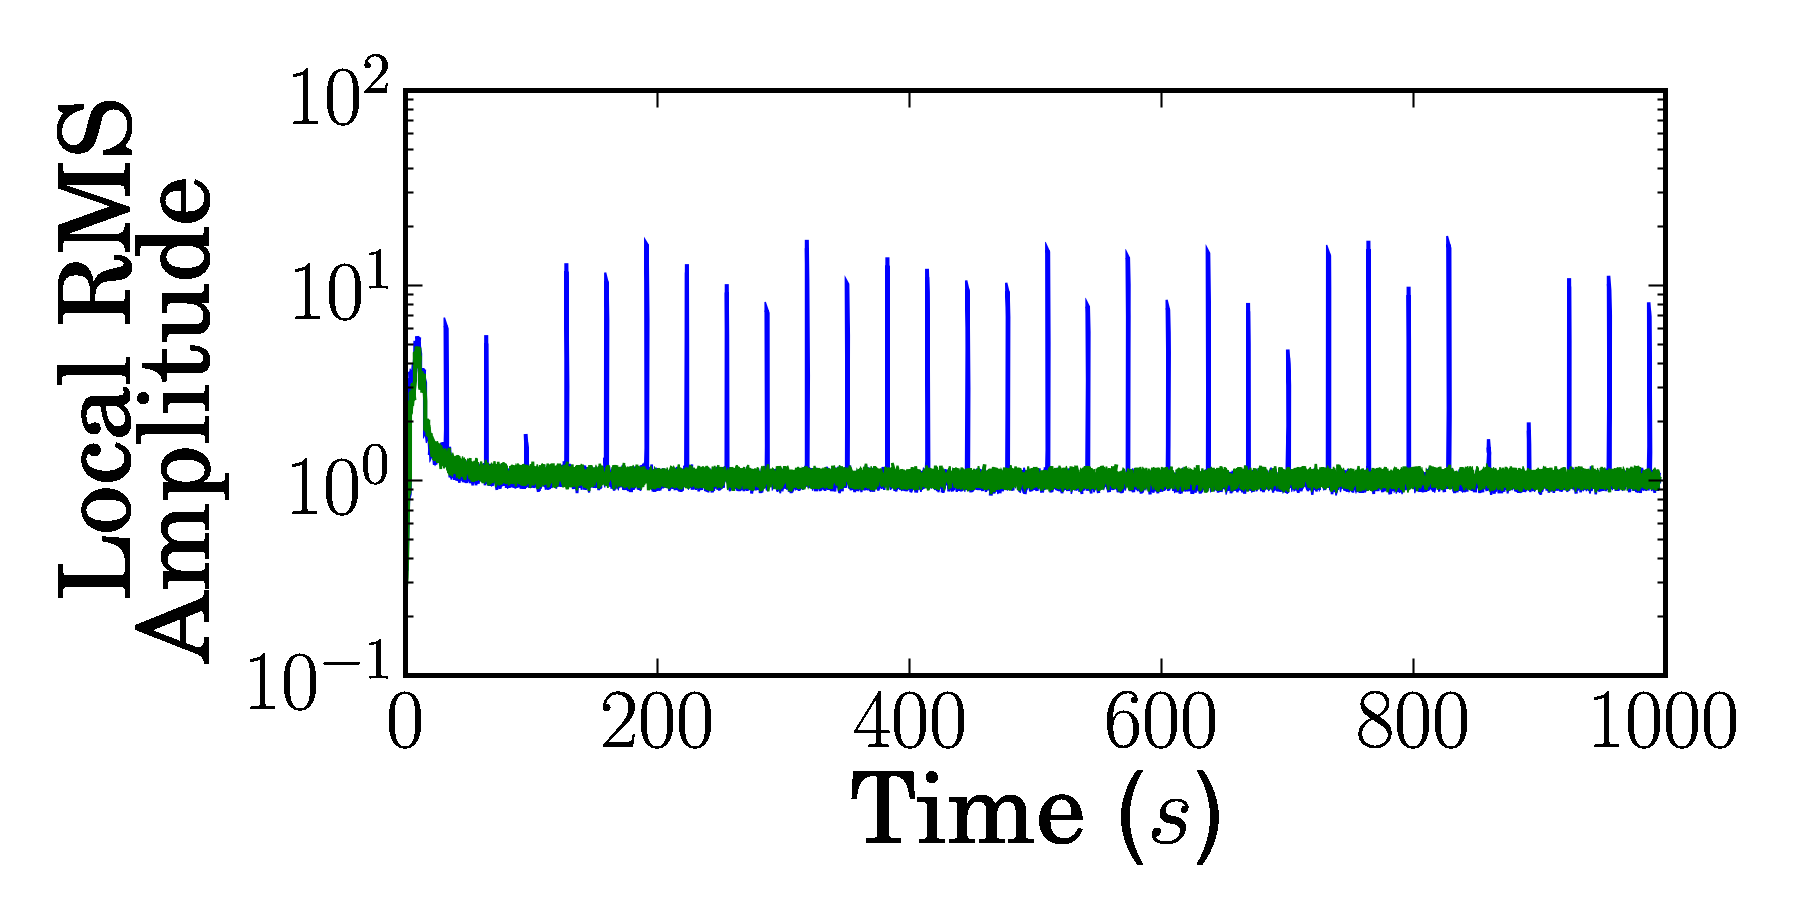
\includegraphics{figures/whiten_burst_step_100_semilogy.png}}
\end{center}

An inspiral, to leading order, has gravitational-wave frequency evolution given
by
\begin{equation}
f(t) = \frac{1}{8 \pi \mathcal{M}} \left( \frac{t_c - t}{5 \mathcal{M}} \right)^{-3/8}\;,
\end{equation}
whose time derivative is given by
\begin{equation}
\frac{df}{dt} = \frac{3}{320 \pi \mathcal{M}^2} \left( \frac{t_c - t}{5 \mathcal{M}} \right)^{-11/8}\;.
\end{equation}
Combining these, we find the frequency evolution as a function of frequency to
be
\begin{equation}
\frac{df}{dt}(f_0) = \frac{3}{320 \pi \mathcal{M}^2} \left( 8 \pi \mathcal{M} f_0 \right)^{3/11}\;,
\end{equation}
which can be inverted to get the minimum frequency which has a given frequency
derivative,
\begin{equation}
f_0 = \frac{1}{8 \pi \mathcal{M}} \left( \frac{320 \pi \mathcal{M}^2}{3} \frac{df}{dt} \right)^{11/3}\;.
\end{equation}

If we allow frequency bins to be affected by an injection only once within the
median history, we need to calculate the corresponding $df/dt$ for our PSD
calculation. An FFT of a buffer with length $T$ will have a frequency
resolution $df = 1/(2T)$. Hann windowing the data and overlapping buffers by
50\% introduces correlations in neighboring frequency bins of the FFT. This
means that we actually want the frequency to change by $df = 3/(2T)$ before the
next PSD calculation, which happens a $dt = T/2$ later, resulting in a minimum
$df/dt = 3/T^2$.

Combining these results we find the lower frequency bound for our injections,
assuming a chirp mass for a binary with $m_1 = m_2 = 1 M_{\odot}$ and $T = 8$
s, is 23 Hz.

We want to compute the equivalent injection density which would be biased as
much as lalapps\_inspiral's PSD estimator, which allows $\sim3$ injections per
2048 seconds. It computes the PSD by breaking the segment up into 16 256 second
chunks. These chunks are then combined into to sets of 8 chunks each. The
median of each set is then averaged across the sets for each frequency bin to
produce the PSD estimate for that 2048 second segment. This procedure results
in an average injection density of 1.5 per 8 PSDs in the median history, which
is comparable to LLOID's 1 per 7 PSDs in the median history. Since LLOID has an
injection history of 7 PSDs which span 32 seconds, this means LLOID can perform
one injection every 32 seconds, or 64 injections per 2048 second segment, more
than an order of magnitude increase in density over lalapps\_inspiral.
\end{comment}
